\section{The Iterator Design Pattern}

\subsection{1. Problem Context}
In software architecture, applications often manage elements stored across multiple disparate data structures. For example, a modern media streaming application may maintain an array-based queue for upcoming tracks, a doubly linked list for play history, and a binary search tree (BST) for genre organization.

Without an abstraction layer, the client application must implement specific traversal logic tailored to each container:
\begin{itemize}
    \item \textbf{Array / Contiguous Vector:} Relies on direct indexed access (\texttt{list[i]}).
    \item \textbf{Linked List:} Relies on node-by-node pointer traversal (\texttt{node->next} or \texttt{node->prev}).
    \item \textbf{Tree / Graph:} Requires recursive or stack-based traversal strategies (e.g., in-order, pre-order, DFS, or BFS).
\end{itemize}

\begin{center}
    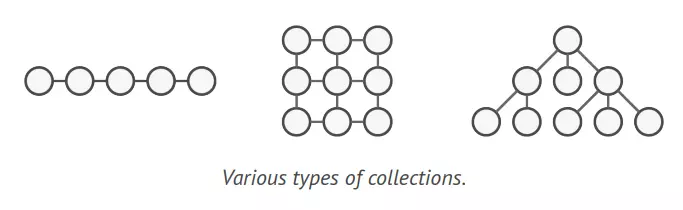
\includegraphics[width=0.7\linewidth]{img/desProblem.png}
\end{center}

\noindent Exposing these low-level traversal mechanisms to consumer code introduces several architectural deficiencies:
\begin{itemize}
    \item \textbf{Encapsulation Leakage:} The internal structure, node pointers, and indexing models of the collection are exposed directly to the client.
    \item \textbf{Single Responsibility Principle (SRP) Violation:} The aggregate class is burdened with managing traversal state and access algorithms in addition to managing its core dataset.
    \item \textbf{Open/Closed Principle (OCP) Violation:} Introducing a new collection type or altering an existing data structure requires updating all client-side traversal loops across the codebase.
    \item \textbf{Code Duplication:} Traversal and rendering algorithms must be rewritten or overloaded for every individual container type.
\end{itemize}

\subsection{2. Solution Architecture}
The \textbf{Iterator Pattern} decouples traversal algorithms from collection data structures by extracting navigation state into an external, dedicated object known as an \textbf{Iterator}. 

\begin{figure}[htbp]
\centering
\begin{verbatim}
+-------------------+                      +---------------------+
|   <<Interface>>   |                      |    <<Interface>>    |
|     Aggregate     |                      |      Iterator       |
+-------------------+                      +---------------------+
| +createIterator() |                      | +hasNext(): bool    |
+---------+---------+                      | +next(): Element    |
          ^                                +----------+----------+
          |                                           ^
+---------+---------+   Creates ConcreteIterator      |
| ConcreteAggregate | - - - - - - - - - - - - - - - ->+---------+
+-------------------+                      |  ConcreteIterator   |
| -collectionData   |                      +---------------------+
| +createIterator() |                      | -cursor / state     |
+-------------------+                      | -aggregateReference |
                                           +---------------------+
\end{verbatim}
\caption{Iterator Pattern Architecture}
\end{figure}

The pattern establishes two primary interface hierarchies:
\begin{enumerate}
    \item \textbf{Aggregate Interface (\texttt{Iterable}):} Defines a factory method (e.g., \texttt{createIterator()}) that supplies a compatible traversal cursor without revealing the internal container layout.
    \item \textbf{Iterator Interface:} Exposes a standard traversal contract—traditionally \texttt{hasNext()} and \texttt{next()}, or \texttt{first()}, \texttt{next()}, \texttt{isDone()}, and \texttt{currentItem()}.
\end{enumerate}

\subsubsection{C++ Implementation Example}
Below is a clean implementation demonstrating an aggregate queue decoupled from its consumer via an iterator interface:

\begin{lstlisting}[language=C++]
#include <iostream>
#include <memory>
#include <vector>
#include <string>

// Target data element
struct Track {
    std::string title;
    std::string artist;
};

// 1. Iterator Interface
class TrackIterator {
public:
    virtual ~TrackIterator() = default;
    virtual bool hasNext() const = 0;
    virtual const Track& next() = 0;
};

// 2. Aggregate Interface
class TrackAggregate {
public:
    virtual ~TrackAggregate() = default;
    virtual std::unique_ptr<TrackIterator> createIterator() const = 0;
};

// 3. Concrete Aggregate
class PlaylistQueue : public TrackAggregate {
private:
    std::vector<Track> tracks;

    // Concrete Iterator as an inner/friend class
    class VectorTrackIterator : public TrackIterator {
    private:
        const std::vector<Track>& items;
        size_t cursor = 0;

    public:
        explicit VectorTrackIterator(const std::vector<Track>& target)
            : items(target) {}

        bool hasNext() const override {
            return cursor < items.size();
        }

        const Track& next() override {
            return items[cursor++];
        }
    };

public:
    void addTrack(const Track& track) {
        tracks.push_back(track);
    }

    std::unique_ptr<TrackIterator> createIterator() const override {
        return std::make_unique<VectorTrackIterator>(tracks);
    }
};

// 4. Client Usage (Uniform Traversal)
void printPlaylist(const TrackAggregate& playlist) {
    std::unique_ptr<TrackIterator> it = playlist.createIterator();
    int index = 1;
    while (it->hasNext()) {
        const Track& t = it->next();
        std::cout << index++ << ". " << t.title 
        << " by " << t.artist << "\n";
    }
}
\end{lstlisting}

\subsection{3. Advantages and Disadvantages}

\subsubsection{Advantages}
\begin{itemize}
    \item \textbf{Strict Encapsulation:} Client code never accesses the internal node pointers or collection arrays directly.
    \item \textbf{Single Responsibility Principle:} Traversal logic and cursor bookkeeping are isolated inside the iterator class, keeping the container focused solely on data storage.
    \item \textbf{Open/Closed Principle:} New data structures or alternative traversal strategies (e.g., filtered, reverse, or breadth-first) can be added without modifying existing consumer loops.
    \item \textbf{Independent Concurrent Traversals:} Because each iterator maintains its own cursor state, multiple independent traversals can run across the same underlying container simultaneously.
    \item \textbf{Lazy Evaluation / Memory Efficiency:} Elements can be processed on-demand, enabling safe traversal of streaming data, infinite sequences, or large database cursors without exhausting memory.
\end{itemize}

\subsubsection{Disadvantages}
\begin{itemize}
    \item \textbf{Over-Engineering for Simple Needs:} Implementing polymorphic interfaces, factory methods, and custom iterator classes introduces unnecessary complexity for simple, fixed-size structures.
    \item \textbf{Indirection Overhead:} Virtual function dispatch and dynamic memory allocations (\texttt{new} / \texttt{std::make\_unique}) introduce minor CPU and heap overhead compared to native index loops.
\end{itemize}

\subsection{4. High-Performance Optimization Techniques in C++}

\subsubsection{Zero-Cost Abstractions and Stack-Allocated Iterators}
In performance-critical C++, virtual method calls and heap allocation can be bypassed entirely by utilizing stack-allocated value types that satisfy the C++ standard range idiom (\texttt{begin()} and \texttt{end()}):

\begin{lstlisting}[language=C++]
class HighPerformanceBuffer {
private:
    std::vector<Track> buffer;

public:
    // Lightweight Stack-Allocated Iterator
    struct Iterator {
        const Track* ptr;

        bool operator!=(const Iterator& other) const { 
            return ptr != other.ptr; 
        }
        const Track& operator*() const { return *ptr; }
        Iterator& operator++() { ++ptr; return *this; }
    };

    Iterator begin() const { return Iterator{buffer.data()}; }
    Iterator end() const { 
        return Iterator{buffer.data() + buffer.size()}; 
    }
};

// Enables compiler-inlined, zero-cost range-based for loops:
void renderAll(const HighPerformanceBuffer& buff) {
    for (const auto& track : buff) {
        std::cout << track.title << "\n";
    }
}
\end{lstlisting}

\subsubsection{Internal Iterators via Higher-Order Functions}
Unlike external iterators where the client drives traversal manually via loops, internal iterators encapsulate loop execution inside the aggregate and apply a callback to each item:

\begin{lstlisting}[language=C++]
class SongCollection {
    std::vector<Track> songs;
public:
    template <typename Callback>
    void forEach(Callback action) const {
        for (const auto& song : songs) {
            action(song);
        }
    }
};
\end{lstlisting}

\subsection{5. Concurrency and Mutation Handling}
Modifying a collection while an iterator is actively traversing it leads to race conditions, invalid iterators, or exceptions. The table below contrasts standard synchronization techniques:

\begin{table}[htbp]
\centering
\caption{Comparison of Thread-Safe Iteration Strategies}
\begin{tabular}{@{}p{3.6cm} p{4cm} p{3.8cm} p{3.2cm}@{}}
\toprule
\textbf{Technique} & \textbf{Mechanism} & \textbf{Advantages} & \textbf{Disadvantages} \\ \midrule
\textbf{Shared Mutex} (\texttt{std::shared\_mutex}) & Uses shared locks for reading/iteration; exclusive locks for writing. & Simple; minimal memory overhead. & High read load can starve pending write operations. \\ \midrule
\textbf{Defensive Snapshot} & Iterator duplicates the underlying collection at creation time. & Eliminates reader-writer conflicts completely. & Allocation and copying overhead proportional to collection size. \\ \midrule
\textbf{Atomic Pointer Swap (Copy-on-Write)} & Traversals read an immutable shared snapshot; writes clone and atomically swap pointers. & 100\% lock-free traversal at native CPU cache speed. & High write-amplification cost on frequent updates. \\ \bottomrule
\end{tabular}
\end{table}

\begin{lstlisting}[language=C++]
#include <iostream>
#include <vector>
#include <memory>
#include <atomic>

class LockFreeTrackCatalog {
private:
    std::atomic<std::shared_ptr<const std::vector<Track>>> 
        catalog_ptr;

public:
    LockFreeTrackCatalog() {
        catalog_ptr.store(std::make_shared<const        
            std::vector<Track>>());
    }

    // Lock-free read traversal: completely 
    immune to concurrent writes
    void traverse() const {
        std::shared_ptr<const std::vector<Track>> 
            snapshot = catalog_ptr.load();
        for (const auto& track : *snapshot) {
            std::cout << track.title << "\n";
        }
    }

    // Write operation using atomic compare-and-swap
    void addTrack(const Track& track) {
        std::shared_ptr<const std::vector<Track>> old_data;
        std::shared_ptr<const std::vector<Track>> new_data;

        do {
            old_data = catalog_ptr.load();
            auto copy = std::make_shared<std::vector<Track>>(*old_data);
            copy->push_back(track);
            new_data = copy;
        } while (!catalog_ptr.compare_exchange_weak(old_data, new_data));
    }
};
\end{lstlisting}

\subsection{6. Real-World Applications}
\begin{itemize}
    \item \textbf{Hierarchical DOM Traversal:} Modern web rendering engines use iterators to traverse recursive DOM trees without exposing internal node linkage.
    \item \textbf{Infinite Scrolling and Pagination:} Mobile and web feeds leverage iterators to paginate remote API data on demand, keeping RAM usage low.
    \item \textbf{Offline Sync Queues:} Mobile systems iterate sequentially through persistent task logs to replay operations after reconnecting to a network.
\end{itemize}

\subsection{7. Relationship with Other Design Patterns}

\subsubsection{Iterator vs. Visitor}
\begin{table}[htbp]
\centering
\caption{Architectural Comparison: Iterator vs. Visitor}
\begin{tabular}{@{}p{3.5cm} p{5.5cm} p{5.5cm}@{}}
\toprule
\textbf{Dimension} & \textbf{Iterator Pattern} & \textbf{Visitor Pattern} \\ \midrule
\textbf{Core Objective} & Access and sequence traversal without exposing internals. & Adding new operations to class hierarchies without modifying their code. \\ \midrule
\textbf{Target Elements} & Homogeneous data structures. & Heterogeneous object hierarchies. \\ \midrule
\textbf{Dispatch Model} & Single dispatch (\texttt{it->next()}). & Double dispatch (\texttt{node->accept(visitor)}). \\ \midrule
\textbf{Control Flow} & External (driven by client loop). & Internal (driven by structural traversal). \\ \bottomrule
\end{tabular}
\end{table}

\noindent \textbf{Synergy:} An Iterator can traverse a complex composite hierarchy sequentially, passing each node to a Visitor that executes polymorphic operations without altering the tree structure.

\subsubsection{Iterator vs. Chain of Responsibility}

\begin{table}[htbp]
\centering
\caption{Architectural Comparison: Iterator vs. Chain of Responsibility}
\begin{tabular}{@{}p{3.5cm} p{5.5cm} p{5.5cm}@{}}
\toprule
\textbf{Dimension} & \textbf{Iterator Pattern} & \textbf{Chain of Responsibility Pattern} \\ \midrule
\textbf{Core Objective} & Traverses elements sequentially across a collection without exposing its internal structure. & Passes a request along a dynamic chain of potential handlers until one processes it. \\ \midrule
\textbf{Flow Control} & Sequential and deterministic; visits every element in order unless explicitly terminated by the client. & Conditional and delegated; execution passes down the handler link until a condition or termination criteria is met. \\ \midrule
\textbf{Decoupling Target} & Decouples the consumer algorithm from the underlying data structure layout. & Decouples the sender of a request from its potential receivers/handlers. \\ \midrule
\textbf{State Management} & Tracks iteration state (cursors, indices, tree pointers) explicitly. & Handlers maintain references only to their immediate successor in the chain. \\ \bottomrule
\end{tabular}
\end{table}

\noindent \textbf{Synergy (Processing Pipelines):}
The two patterns frequently collaborate in data processing pipelines, middleware stacks, and stream filtration:
\begin{itemize}
    \item The \textbf{Iterator} acts as the \textit{data source pump}, fetching items one-by-one from complex, memory-efficient data structures without exposing internal node layouts.
    \item The \textbf{Chain of Responsibility} acts as the \textit{processing pipeline}, routing each item produced by the iterator through a series of discrete, loosely coupled validation, filtering, or transformation stages.
\end{itemize}

\begin{lstlisting}[language=C++]
#include <iostream>
#include <memory>
#include <string>
#include <vector>

struct Track {
    std::string title;
    int durationSec;
    bool isExplicit;
};

// --- CHAIN OF RESPONSIBILITY: Handler Interface ---
class TrackFilter {
protected:
    std::shared_ptr<TrackFilter> nextHandler;

public:
    virtual ~TrackFilter() = default;

    void setNext(std::shared_ptr<TrackFilter> next) {
        nextHandler = next;
    }

    virtual bool process(const Track& track) {
        if (nextHandler) {
            return nextHandler->process(track);
        }
        return true; // Passed all pipeline stages
    }
};

// Concrete Handler 1: Filter explicit content
class ExplicitFilter : public TrackFilter {
public:
    bool process(const Track& track) override {
        if (track.isExplicit) {
            std::cout << "[Blocked - Explicit]: " << track.title << "\n";
            return false;
        }
        return TrackFilter::process(track);
    }
};

// Concrete Handler 2: Filter out short tracks (< 30 seconds)
class DurationFilter : public TrackFilter {
public:
    bool process(const Track& track) override {
        if (track.durationSec < 30) {
            std::cout << "[Skipped - Too Short]: " << track.title << "\n";
            return false;
        }
        return TrackFilter::process(track);
    }
};

// --- ITERATOR + CHAIN OF RESPONSIBILITY IN ACTION ---
void runAudioPipeline(TrackIterator& it, TrackFilter& pipeline) {
    std::cout << "--- Processing Tracks Through Filter Pipeline ---\n";
    while (it.hasNext()) {
        const Track& track = it.next();
        // Iterator provides the item; Chain processes/filters the item
        if (pipeline.process(track)) {
            std::cout << "[Playing]: " << track.title << "\n";
        }
    }
}
\end{lstlisting}